
%%%%%%%%%%%%%%%%%%%%%%%%%%%%%%%%  ejemplo.tex %%%%%%%%%%%%%%%%%%%%%%%%%%%%%%%

%%%%% Fichero de ejemplo LaTeX que ilustra el uso de la Hoja de Estilo %%%%%%
%%%%% Jornadas.cls para Jornadas Sarteco.              %%%%%%

\documentclass[twocolumn,twoside]{Jornadas}
\usepackage[latin1]{inputenc}
%\usepackage[dvips]{epsfig}

\usepackage{hyperref}
\usepackage{csvsimple}
\usepackage{array}
\usepackage{graphicx}
\usepackage{epstopdf}

\def\BibTeX{{\rm B\kern-.05em{\sc i\kern-.025em b}\kern-.08em
    T\kern-.1667em\lower.7ex\hbox{E}\kern-.125emX}}

\newtheorem{theorem}{Teorema}


\newcolumntype{L}[1]{>{\raggedright\let\newline\\\arraybackslash\hspace{0pt}}m{#1}}
\newcolumntype{C}[1]{>{\centering\let\newline\\\arraybackslash\hspace{0pt}}m{#1}}
\newcolumntype{R}[1]{>{\raggedleft\let\newline\\\arraybackslash\hspace{0pt}}m{#1}}


%%%%%%%%%%%%%%%%%%%%%%%%%%%%%%%%%%%%%%%%%%%%

\hyphenation{pa-ra-le-lis-mo pro-cee-dings de-ma-sia-do Su-ge-ri-mos
             mo-di-fi-ca-cio-nes afi-lia-cio-nes re-fe-ren-te co-men-ta-rios
             usan-do pro-ble-ma plan-ti-lla}

\begin{document}


\title{Studying individualized transit indicators using a new low-cost information system}

\author{%
    P.A. Castillo, A. Fern�ndez-Ares, P. Garc�a-Fern�ndez, P. Garc�a-S�nchez, M.G. Arenas, A.M. Mora, V.M. Rivas, J.J. Asensio, G. Romero, J.J. Merelo
     \thanks{Department of Architecture and Computer Technology. CITIC. University of Granada. Spain. e-mail: {\tt \{ meter los emails \} @ugr.es}}    
}

\maketitle
% Oculta las cabeceras y los n\'umeros de p\'agina.
% Ambos elemetos se a\~nadir\'an durante la edici\'on de las actas completas.
\markboth{}{}
\pagestyle{empty} 
\thispagestyle{empty} % Oculta el n\'umero de la primera p\'agina


\begin{abstract}
Current information systems used for data collection and to generate information on the state of the roads
have two drawbacks: the first is that they have no ability to identify and target detected vehicles. The
second is their high cost, which makes them expensive to cover the secondary road network, so they are
usually located just on main routes. Thus, a new low-cost information system to monitor the traffic in
real-time is proposed. This system is based on scanning Bluetooth devices that are near the detection
node. A large amount of data from passes of Bluetooth devices by different nodes (movements or
displacements) have been collected. From this data, the frequency of appearance, average speed, or the
number of devices that pass a certain site each day (on both working or non-working days) can be
determined. The analysis of collected data has given statistics and indicators about the use of vehicles by
the population of the monitored area. Specifically, we have obtained information about the total number
of vehicles that each node has detected, on weekdays or holidays, information on traffic density by time
range, on individual movements, and the average speed on a section delimited by two consecutive nodes,
what demonstrates the power and features of the developed system.
\end{abstract}

\begin{keywords}
Traffic flow, time series forecasting, evolutionary computation, artificial neural networks
\end{keywords}

\section{Introducci�n}
\PARstart{N}{owadays}, having a system of information on traffic conditions and the use of roads is very important, not only to obtain information about traffic density, but also about repetitions of passing vehicles. This kind of information about traffic flows that occur in a certain area could allow people to optimally manage their motion decisions.

Current technologies used in traffic monitoring include pneumatic tubes, loop detectors, floating vehicles or automatic recognition systems, among others. The main disadvantage of these systems is that they are unable to identify detected vehicles, in order to obtain origin/destination matrixes. Just the number of vehicles and their type can be obtained, but they do not allow to obtain traffic flow, nor to determine whether a certain vehicle passes repeatedly. In addition, their high cost makes it unprofitable covering secondary roads with them, so they are often located on major roads. Moreover, technologies based on video image detection are very costly compared to the previous and can be sensitive to meteorological conditions.

In this work, several individualized transit indicators are studied using a new low-cost system information, with a fast deployment and highly reliable. This system provides real-time information about the traffic status on different road types and in real time (available as web services), not only to the official organisms and agencies in charge of the traffic controlling, but also to any person who requests it.

Our aim is having information about traffic using a new system based on the Bluetooth (BT) devices detection using several collecting nodes. Thus, we are able to monitor the traffic density and car journeys, identifying the vehicles when they move from one node to another inside the monitored zone. Therefore, various needs have been found:

As stated, the proposed system is based on BT device discovery. Specifically, it detects waves emitted by different technological components incorporated on vehicles (hands-free phone sets, GPS) or accessories that the users incorporate to their vehicles, as well as their mobile phones. Although not all vehicles carry a BT transmitter, nowadays increasingly more and more vehicles are equipped with them. In addition, in a very high percentage of vehicles the driver might carry a mobile with BT. In any case, as stated in \cite{Blobject} an a priori error estimation of 8.5\% of detections was obtained.

The system collects the MAC address of the device BT card as well as the exact time at which it has been detected. The MAC is an unique identifier for each device, allowing us to identify passing vehicles. Additionally, analyzing the MAC allows us to determine the manufacturer and even distinguish what type of device it is (i.e. handsfree, PC, mobile phone, etc), as detailed in \cite{IEEEBT} and \cite{wikiOUI}.

From the point of view of data privacy, it is noteworthy that the data collected cannot be associated, at least without recurring to other methods, to any vehicle since there is no information collected that enables the association of the information we collect with a specific person. Unidirectional encryption technology is used, using nonstandard characters that preclude identifying the MAC of the wireless device.

Proposed system is part of a future prediction system that helps to make decisions, and able to apply knowledge in applications related to mobility. It is expected that the development and deployment of these systems will offer a set of information services with added value that are not achieved with current technologies.

The rest of the chapter is organized as follows: following section reviews current technologies to monitor the traffic that passes through a certain area, as well as similar commercial products. Section \ref{sec:objectives} details the goals of this chapter. In section \ref{subsec:devices}, the Intelify device is presented. In section \ref{sec:data} several analysis and statistics are reported from the data obtained. Finally, we present some conclusions and future work. 

\section{Current technologies}
\label{sec:tech}
Nowadays, several technologies are used to data collection and generation of information on the state of the roads and traffic monitoring. Those systems can be classified according to the immediacy of data, completeness in the collection and intrusiveness \cite{martin2003detector}.

According to the immediacy of data collection, systems are classified into direct data collection (the source obtains data experimentally), and indirect data collection (the data is obtained by further processing algorithms).

Taking into account the completeness of data collection, systems can be making nearly exhaustive (the number of measurements taken match the number of users), or non-exhaustive data collection (measurements related to a limited number of users are taken).

Finally, current monitoring technologies can be classified as intrusive technologies (installed in the pavement), not-intrusive technologies (no contact with the road, causing minimal effect on traffic flow), and floating vehicle technologies.

Figure \ref{fig:f1} shows a classification of information systems according to the intrusiveness of the technology.

\begin{figure}[ht]
\begin{center}
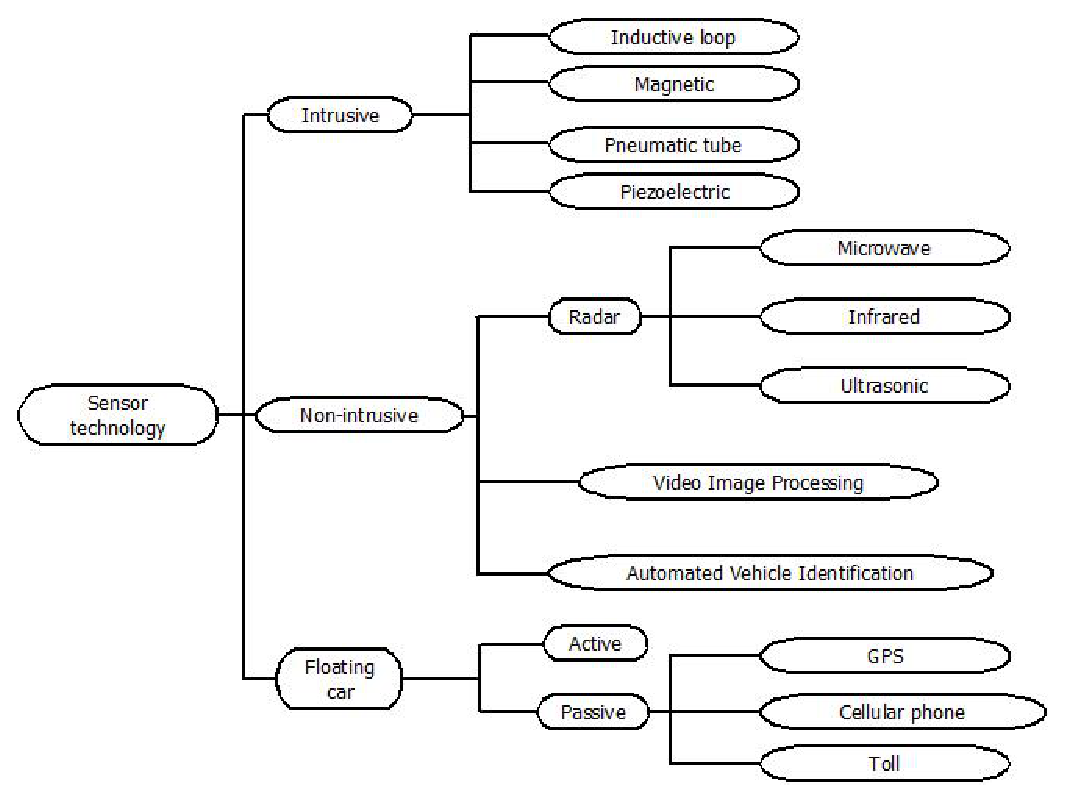
\includegraphics[scale=0.4]{images/Figure_1}
\caption{Information systems classification, according to the intrusiveness of the technology.
\label{fig:f1}}
\end{center}
\end{figure}



Main technologies currently used in traffic monitoring include pneumatic tubes, loop detectors, floating vehicles or automatic recognition systems, among others \cite{rodrigue2013geography}.

Pneumatic tubes are placed on top of the lane to detect vehicles by the change in pressure generated when a vehicle passes over the tube. A device at the roadside counts vehicles. The main drawback is that its efficiency is subject to weather, temperature and traffic conditions.

A loop detector is a wire embedded into the roadway in a square configuration. A device at the roadside records the number of detected vehicles as they induce an electrical current when passing over the wire. Both the implementation and maintenance costs can be expensive.

The use of so-called floating vehicles consists on a vehicle provided with sensors to collect information while driving on a predefined route. This active device data collection is one of the most popular among operators of roads, used especially for the collection of travel time and for loop detector calibration. Depending on the level of automation in the data collection, the cost can vary.

The main disadvantage of these systems is that they are unable to identify detected vehicles, in order to obtain origin/destination matrixes. Just the number of vehicles and their type can be calculated, but does not allow to obtain traffic flow, nor to determine whether a certain vehicle passes repeatedly. In addition, their high cost makes it unprofitable covering secondary roads with them, so they are often located on major roads.


Finally, the automatic recognition technology has experienced an increase in recent years due to its ability to detect individual vehicles without relying on in-vehicle systems. Video image detection is a good example; in this case trip line and/or tracking are used to record traffic data. Furthermore, they are used for automatic detection of incidents on the road. That is the main advantage over previous information systems. However, system reliability might not be the best, as weather may limit accuracy. Moreover, these systems are very costly compared to the previous \cite{skszek2001state}. Finally, from a privacy point of view, the Spanish Data Protection Agency (Agencia de Protecci�n de Datos) considers the car license plate as a personal data, so that it would require the user consent.

\section{Comercial products}
\label{sec:products}
There are different companies working in the traffic information area using approaches similar to the presented in this work:
\begin{itemize}
\item Bit Carrier \cite{mendez2011system,BitCarrier}: It offers a traffic management system based in BT to count people and commercial routes (pathsolver). Its technology was deployed in highways managed by Abertis for traffic control and monitoring. Actually it has a 150 devices network in Catalonia, so it allows count the traffic times of 200.000 persons each day.
\item Trafficnow \cite{Trafficnow}: Another BT system product. A pilot experience has been deployed in Vigo.
\item Traffax Inc \cite{TraffaxInc}: It is a company that also has used BT for calculating origin-destination and transport time matrixes.
\item Savari Networks \cite{SavariNetworks}: It offers the commercial product StreetWAVE for traffic monitoring to know in real time the traffic status.
\item TrafficCast \cite{TrafficCast}: They have developed prediction models in different cities based on different technologies, such as cameras, BT and RFID included in the vehicles.
\end{itemize}
The proposal presented in this work has some common features with the previous approaches, offering similar functionalities with reduced cost.

\section{Objectives and expected results}
\label{sec:objectives}
The main objective was building a low-cost system to provide real-time information about the traffic status and flows that occur in a certain area, allowing to optimally manage motion decisions by citizens.

Thus, several features have been developed:
\begin{itemize}
\item Data collection component: it includes several sensors to continuously scanning and identifying BT devices. It uses a 3G connection to send data to the storage server. It is enclosed in hermetic boxes and uses a 220V power line.
\item Data processing component: it stores the obtained data, and offers some tools to serve them (through web services).
\item Information service: it provides the users the requested information related to the traffic status.
\end{itemize}

Six devices were installed for data collection. They send obtained data to servers for further data processing. Node locations are shown in the map on Figure \ref{fig:f2}. Locations were set according to the suggestions of the National Department of Traffic (DGT), looking for an adequate place, with a continuous flow of vehicles, and also taking into account the assembly difficulty of the monitoring devices.

\begin{figure}[ht]
\caption{Geographical node locations in the metropolitan area of Granada. Source: \url{http://bit.ly/SQdQkH}}
\label{fig:f2}
\begin{center}
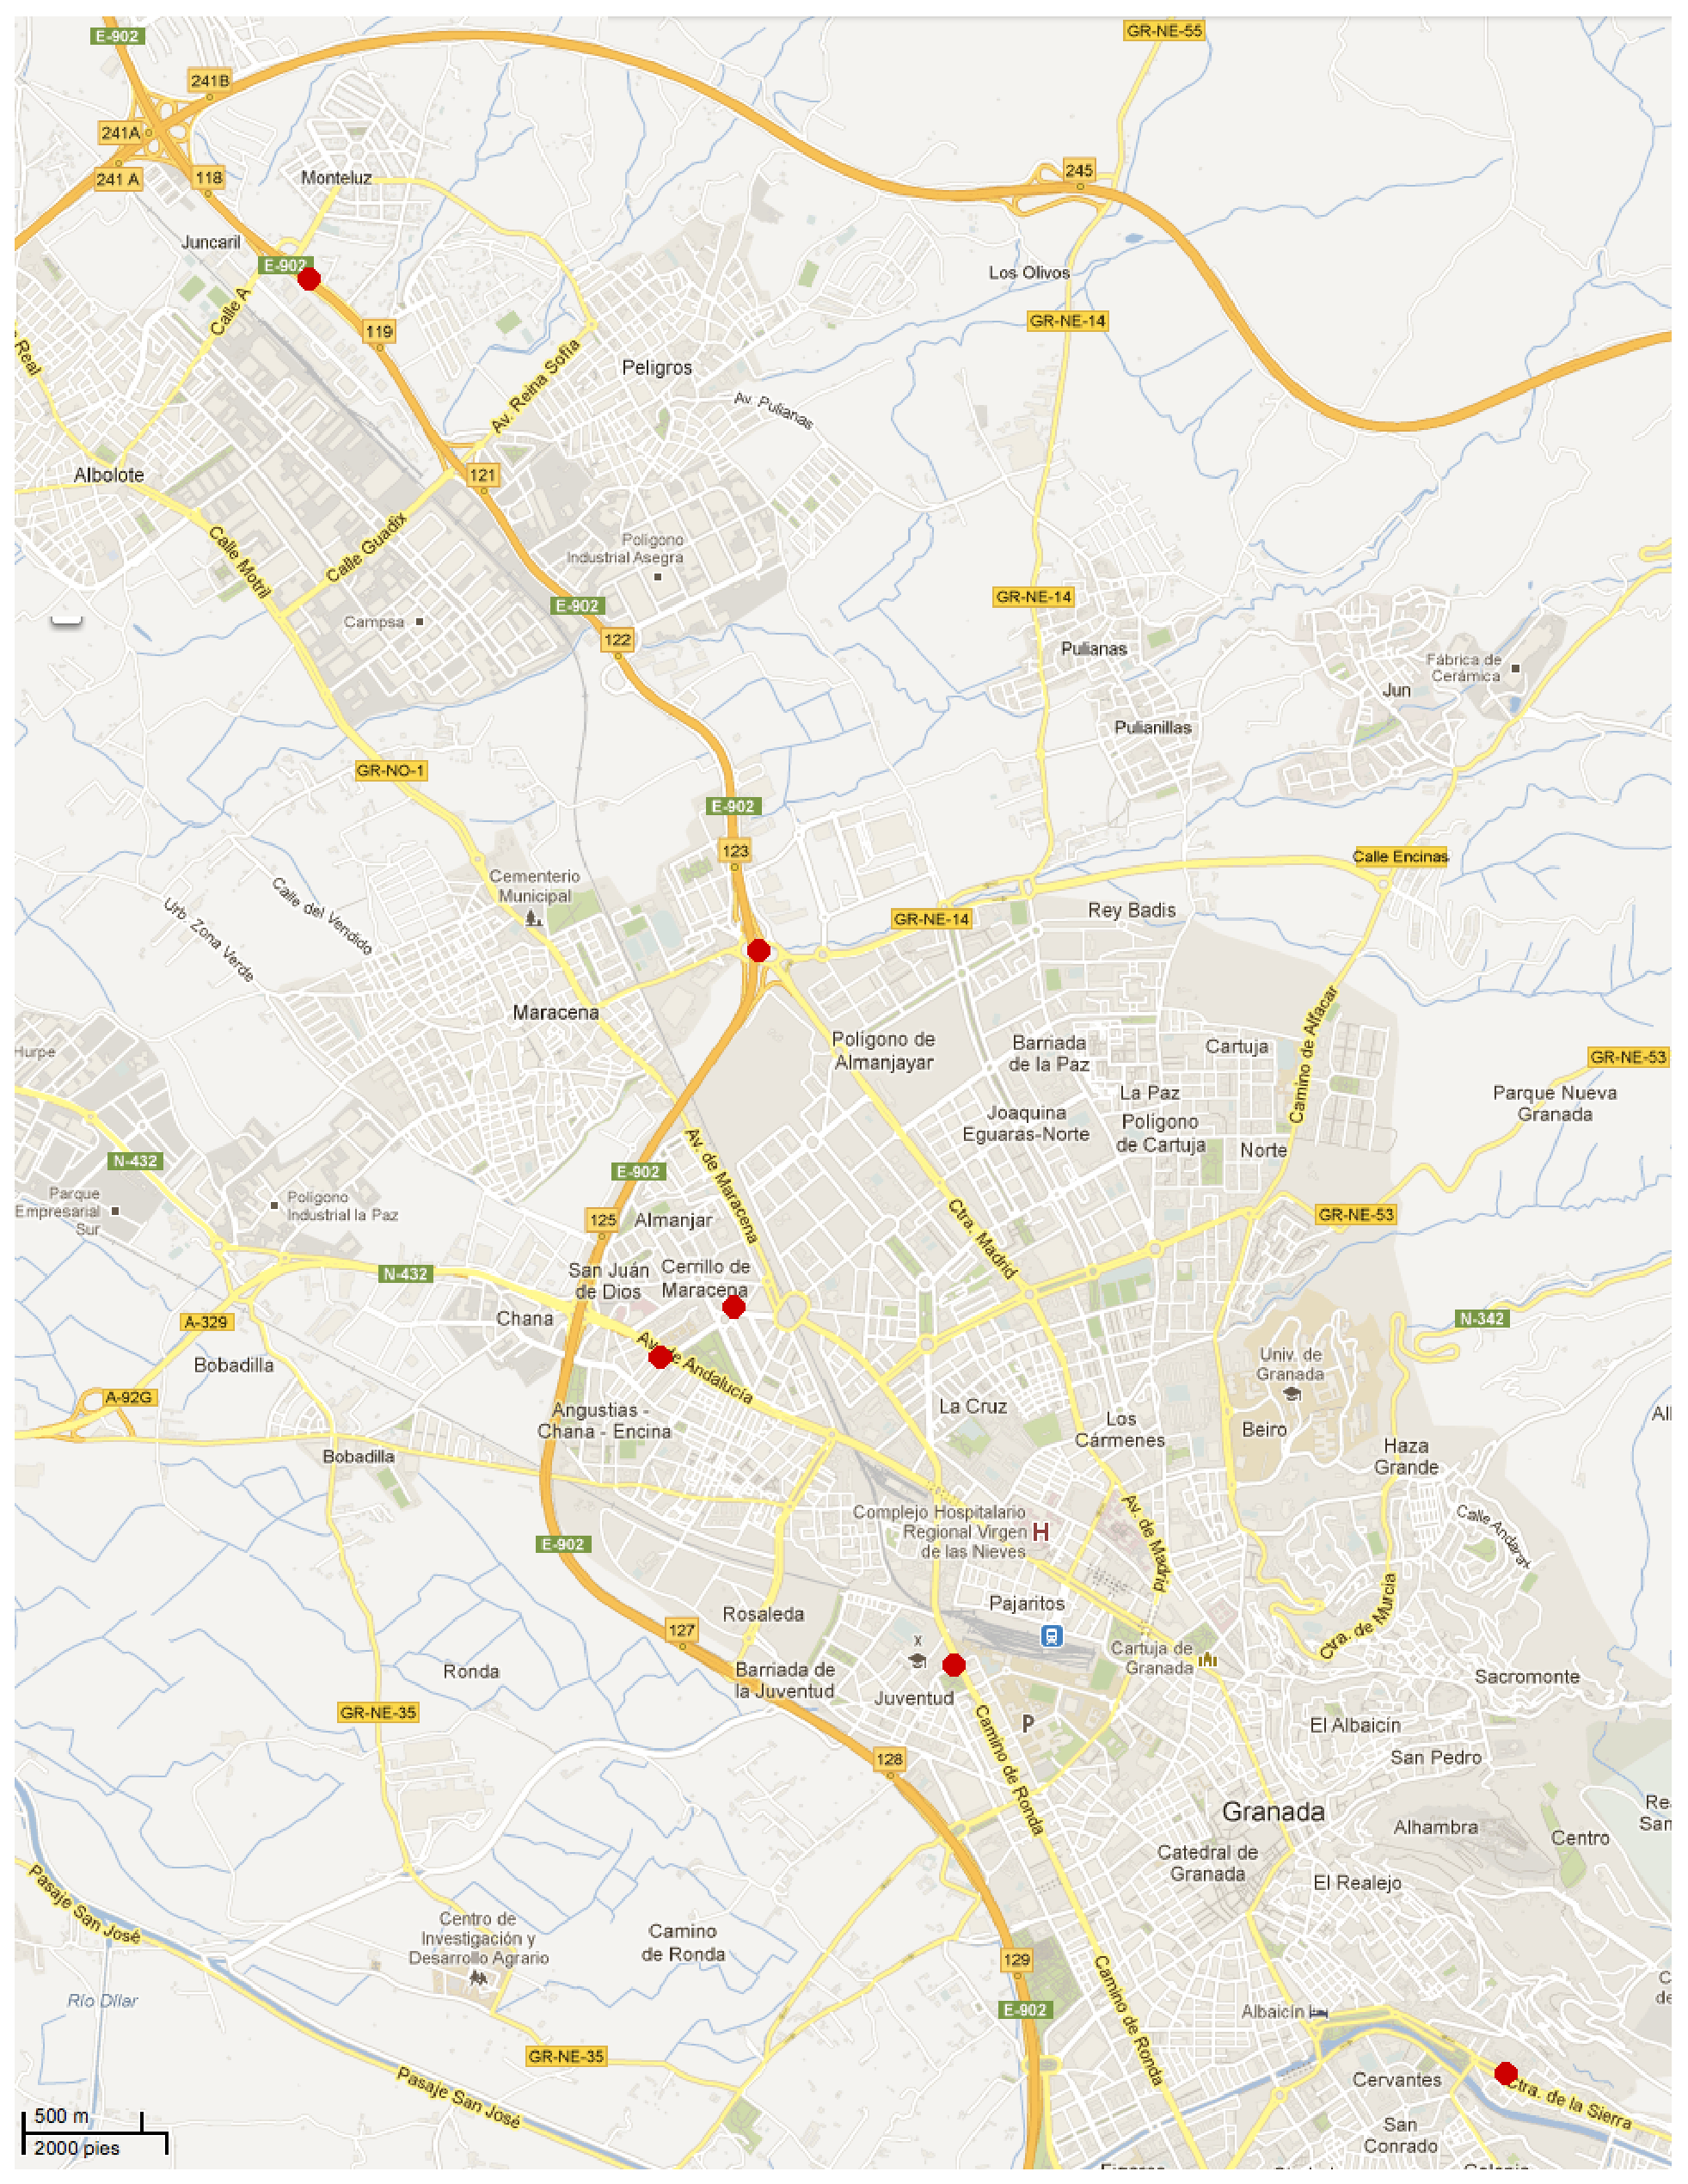
\includegraphics[scale=0.25]{images/Figure_2}
\end{center}
\end{figure}


A large amount of data corresponding to passing BT devices are collected, to populate a big database and to compute different statistics and indicators on the use of vehicles on the monitored area, driving habits and even the effect of important factors or events (key dates, nonworking days, etc).

Specifically, following statistics will be reported:
\begin{itemize}
\item Total amount of detected vehicles by every node.
\item Total amount of detected vehicles in working days.
\item Total amount of detected vehicles in non-working days.
\item Number of times each vehicle is detected.
\item Type of path the vehicles follow.
\item Traffic density by time range and road type.
\item Average speed in the road where two devices where set.
\end{itemize}

\subsection{Data-collecting hardware device}
\label{subsec:devices}
The first step of this study was to choose between several hardware devices to scan for BT devices. First tests were conducted on a PC with Linux and a BT module. This solution was quickly discarded because of its high size and power consumption (see Table \ref{table:comparison}).

Another possible solution studied was using Android cell phones. These are low power consumption devices, with high connectivity, highly available development tools and powerful processors.

A prototype application was developed for Android. The application was limited to three tasks: BT device discovery, BT identification and data sending to a server through its 3G connection. The server finally stored that information in a database. Both the Android application \footnote{\scriptsize{\url{http://sipesca.ugr.es/download/descargas/sipesca_bt.apk}}} and its source code\footnote{\scriptsize{\url{http://sipesca.ugr.es/download/descargas/com.pacv.bt.sipesca1__SRC.zip}}} are available for download.



Despite the advantages of the cell phone, they include small and low power BT antennas. Because of that, their detection capability is very limited; thus, using cell phones was discarded.

Finally the Intelify \cite{Intelify} (see Figure \ref{fig:f3}) was chosen due to its low power consumption and high detection range.

\begin{figure}[ht]
\caption{Intelify device with a connected USB 3G dongle.}
\label{fig:f3}
\begin{center}
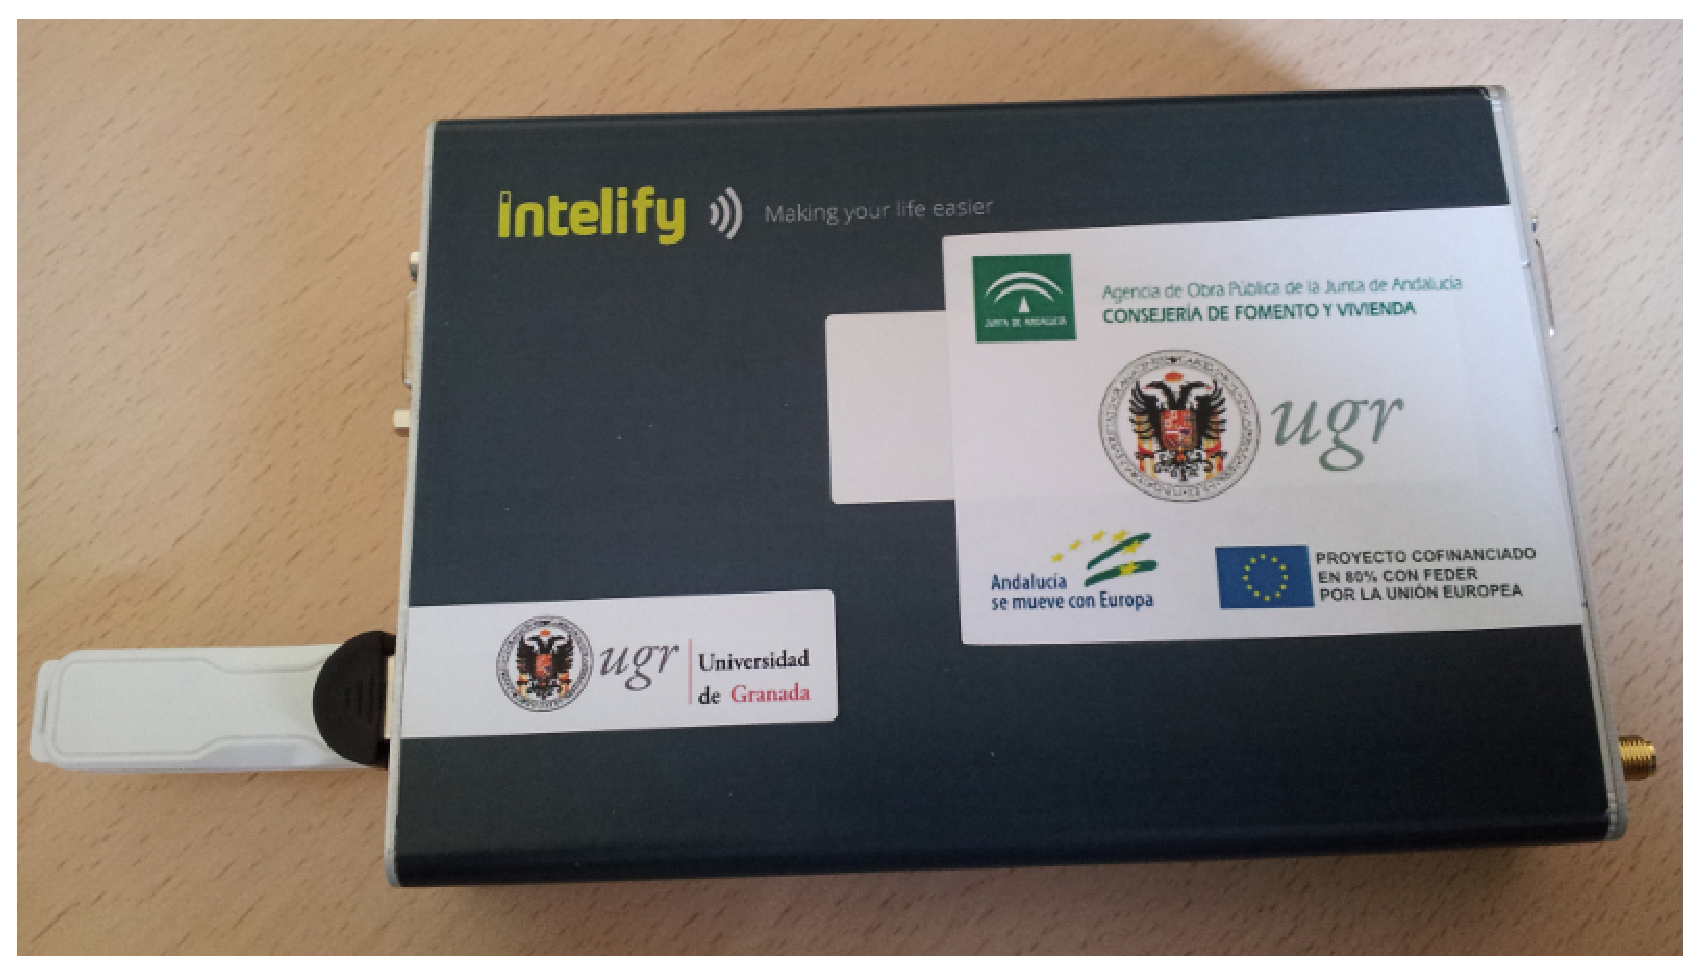
\includegraphics[scale=0.2]{images/Figure_3}
\end{center}
\end{figure}


Intelify is a hardware detection device based on technology developed by Ciudad 2020 \cite{CityAnalytics,Ciudad2020}. It is an autonomous unit that scan the environment and sends the information to a central server for further processing and interpretation. Table \ref{table:features} shows main features of this device.


\begin{table}
\caption{Main features of the Intelify device.}
\label{table:features}
\begin{center}


%\resizebox{5cm}{!}{
\begin{tabular}{|C{2cm}|C{4cm}|}\hline %
\bfseries Feature & \bfseries Description 
\\\hline
\csvreader[head to column names, late after line=\\\hline]{DeviceFeatures.csv}{}%
{\feature & \description}% 
\end{tabular}
%}
\end{center}
\end{table}

For the shake of comparison, Table \ref{table:comparison} shows detailed information about the hardware devices analyzed for data collecting in terms of size and power consumption. Given the power and low-consumption of the Raspberry-Pi platform \cite{wikiRBP}, nowadays a new monitoring device based on this new platform is under development. 


\begin{table}
\small
\caption{Comparison of the hardware devices analyzed for data collecting in terms of size and power consumption.}
\label{table:comparison}
\begin{center}
\begin{tabular}{|C{2.5cm}|C{1cm}|C{2.5cm}|}\hline 
\bfseries Device & \bfseries Power  & \bfseries Dimensions
\\\hline
\csvreader[head to column names, late after line=\\\hline]{DeviceComparison.csv}{}
{\device & \consumption & \dimensions} 
\end{tabular}
\end{center}
\end{table}


Intelify is a small autonomous computer that can be installed in any area to be monitored. It has several sensors that let you discover what is happening in its surroundings like the flow of people and vehicles.

Device operation is based on scanning devices that are in the area of the BT antenna range using the hcitool operating system tool. This tool is used to configure BT connections and send special commands to BT devices. For example, to discover the BT-enabled devices within range, we can use the scan command:
hcitool scan
hcitool will display the list of MAC addresses of the discovered devices.

Technology was developed by Ciudad 2020 and the services offered are based on a net of monitoring devices with the capacity to discover information about the physical environment and help with decision making to any kind of organization based on people flow and behavior. Valuable information about tourism, trade and mobility can be gathered through the deployment of these autonomous devices around a city. 


The cost of this solution is under \$ 1000 per device, including remote maintenance, communications using a 3G service, storage and data management.
Data accuracy is very representative, as stated previously, having obtained an a priori error estimation of 8.5\% of detections \cite{Blobject}.

\subsection{Sharing data and information using web services}

To allow the integration with other systems, the Service Oriented Paradigm \cite{papazoglou2007service,garcia2010distributed} has been used. This paradigm allows the usage of available service interfaces (usually over Internet) to access to required information. 

These interfaces allow the "service consumers" to interact "service implementations" with independence of the programming language or operating systems \cite{arsanjani2008soma,castillo2012distributed}. Implementations can be changed and updated, allowing the interoperability and integration with other systems.

Whatever the technology used to deploy web services, they provide several advantages, like language independence and distribution mechanisms; it also increases the interoperability between different software elements (for example, it is possible to add communication libraries without modifying existing code), and facilitates code distribution (it is not required the use of a concrete implementation or library) among geographically distributed work teams \cite{castillo2013using}.

In this case, our platform uses Representational State Transfer (REST) web services \cite{fielding2000architectural}\cite{fielding2002principled}\cite{Vinoski200884}, as this paradigm adheres much more closely to a web-based design. REST is an alternative method for building web services. This technology was proposed and defined by Roy Fielding  \cite{fielding2000architectural}\cite{fielding2002principled}. In a REST-style architecture, a client sends requests to the server who process them and return responses to the client. Requests and responses represent resources that can be addressed by an Uniform resource identifier (URI). Usually, resources are documents or programs the client need to access to.

REST web services are simple and lightweight (as no extra XML markup is needed), their message format is readable by humans, they are easy to build, and finally, developments achieve a high performance \cite{daigneau2011service}.


\subsection{Data services implementation}

Developed data services have been designed to extract/insert information in the database taking into account security and availability requirements. Among the different web-centered data management systems Google web services, specifically Google Fusion Tables \cite{gonzalez2010google}\cite{gonzalez2010socializing} was chosen to serve information to end users.  

Google Fusiont Tables is built on two layers:
\begin{itemize}
\item Bigtable: the tuples of pairs (key, value) are sorted on the key and sharded among multiple servers based on key ranges. Bigtable provides a write operation that inserts a new tuple automatically and three read operations to retrieve pairs, namely by key, by key prefix or by key range. For each tuple a transaction-time history is recorded.
\item Megastore: On top of bigtable Megastore provides higher level primitives such as consistent secondary indexes, multi-rows transactions, and consistent replication.
\end{itemize}


The motivation for this choice is based on the following features:

\begin{itemize}
\item Export and attribution: We can restrict the ability of others to export the data outside Fusion Tables. We can also control who we share the data with and the data is always carring around the attribution, no matter what transformation gets applied.
\item Search: the public data is made discoverable by search engines, so they can direct users to the data when this is relevant to their queries.
\item Sharing and integration: data can be shared between organizations and can be merged from multiple owners.
\item Visualization: Fusion Tables offers serveral map viewing options for geographic location values and useful visualizations of time data values which occur frequently in our services.
\end{itemize}

Thus, we ensure the availability of information to users, and at the same time we reduce our server load. This way, users can access our database with an extra layer of security and management (instead accessing the database directly). 

This mechanism, and therefore allowing the usage of our system data by third parties, will facilitate the easy creation of web pages and mobile apps to serve useful information to the users.

In this sense, a cross-platform mobile application to allow users access any kind of data using computers, mobile phones and tablets is under development. Figure \ref{fig:f4} shows several screenshots of this application. Both the application\footnote{\url{http://sipesca.ugr.es/download/descargas/sipesca_info.apk}} and its source code\footnote{\url{http://sipesca.ugr.es/download/descargas/com.pacv.info.sipesca1__SRC.zip} } are available for download.

\begin{figure}[ht]
\caption{Screenshots of the Android application developed to serve information to the users.}
\label{fig:f4}
\begin{center}
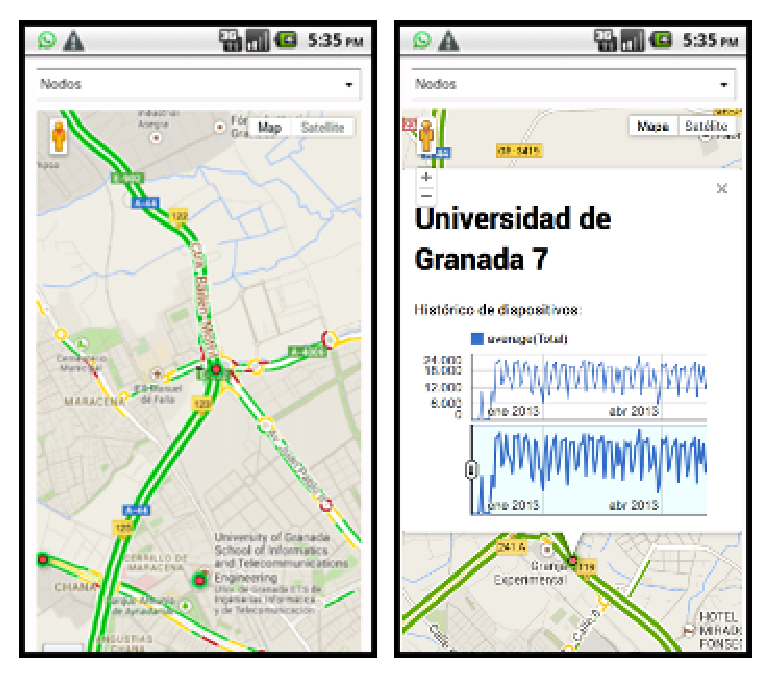
\includegraphics[scale=0.6]{images/Figure_4}
\end{center}
\end{figure}

\section{Data analisys}
\label{sec:data}
In this section the analysis of collected data during the monitoring period (November 8 to December 9, 2012) to obtain statistics and so study the use of vehicles is carried out.

Specifically, the following subsections report information about the total number of detected vehicles by each node, on weekdays or holidays, information on traffic density by time range and the average speed on a section delimited by two consecutive nodes.
\subsection{Total number of detected vehicles (in weekdays and holidays)}
The first analysis consisted in calculating the number of detected devices per node.

\begin{table}
\caption{Number of BT detected devices per node.}
\label{table:detections1}
\begin{center}
\begin{tabular}{|R{2cm}|R{3cm}|}\hline 
\bfseries  \makebox[2cm][c]{Node Id.} & \bfseries  \makebox[3cm][c]{N. of devices}
\\\hline
\csvreader[head to column names, late after line=\\\hline]{NodeDetections1.csv}{}
{ \nodeid & \detections }
\end{tabular}
\end{center}
\end{table}

About 773845 BT devices have been detected in total. As shown in Table \ref{table:detections1}, nodes located in the Sierra Nevada Highway (A44, nodes 4 and 5) have collected a higher amount of data, while the node located in a side street (node 6) has detected the smallest amount of devices.

\subsection{Total detected vehicles in non-working days}
To compare the traffic intensity between working and non-working days, the number of passes in holidays and non-working days have been obtained.

\begin{table}
\caption{Total number of BT detected devices per node (only in non-working days).}
\label{table:detections2}
\begin{center}
\begin{tabular}{|R{2cm}|R{3cm}|}\hline 
\bfseries  \makebox[2cm][c]{Node Id.} & \bfseries  \makebox[3cm][c]{N. of devices}
\\\hline
\csvreader[head to column names, late after line=\\\hline]{NodeDetections2.csv}{}
{ \nodeid & \detections }
\end{tabular}
\end{center}
\end{table}

Table \ref{table:detections2} shows how the number of detected devices is reduced in all nodes in non-working days, compared to the number of detections in weekdays. Nodes located in the Sierra Nevada Highway still collected much more data than the remainder, due to the traffic this road supports on holidays.

\subsection{Traffic density on the road by time range}
Traffic density can be calculated taking into account the total number of detected devices by time range.

\begin{figure}[ht]
\caption{For each node, the total number of different detected devices by time range is shown. Figure is shown in logarithmic scale.}
\label{fig:f5}
\begin{center}
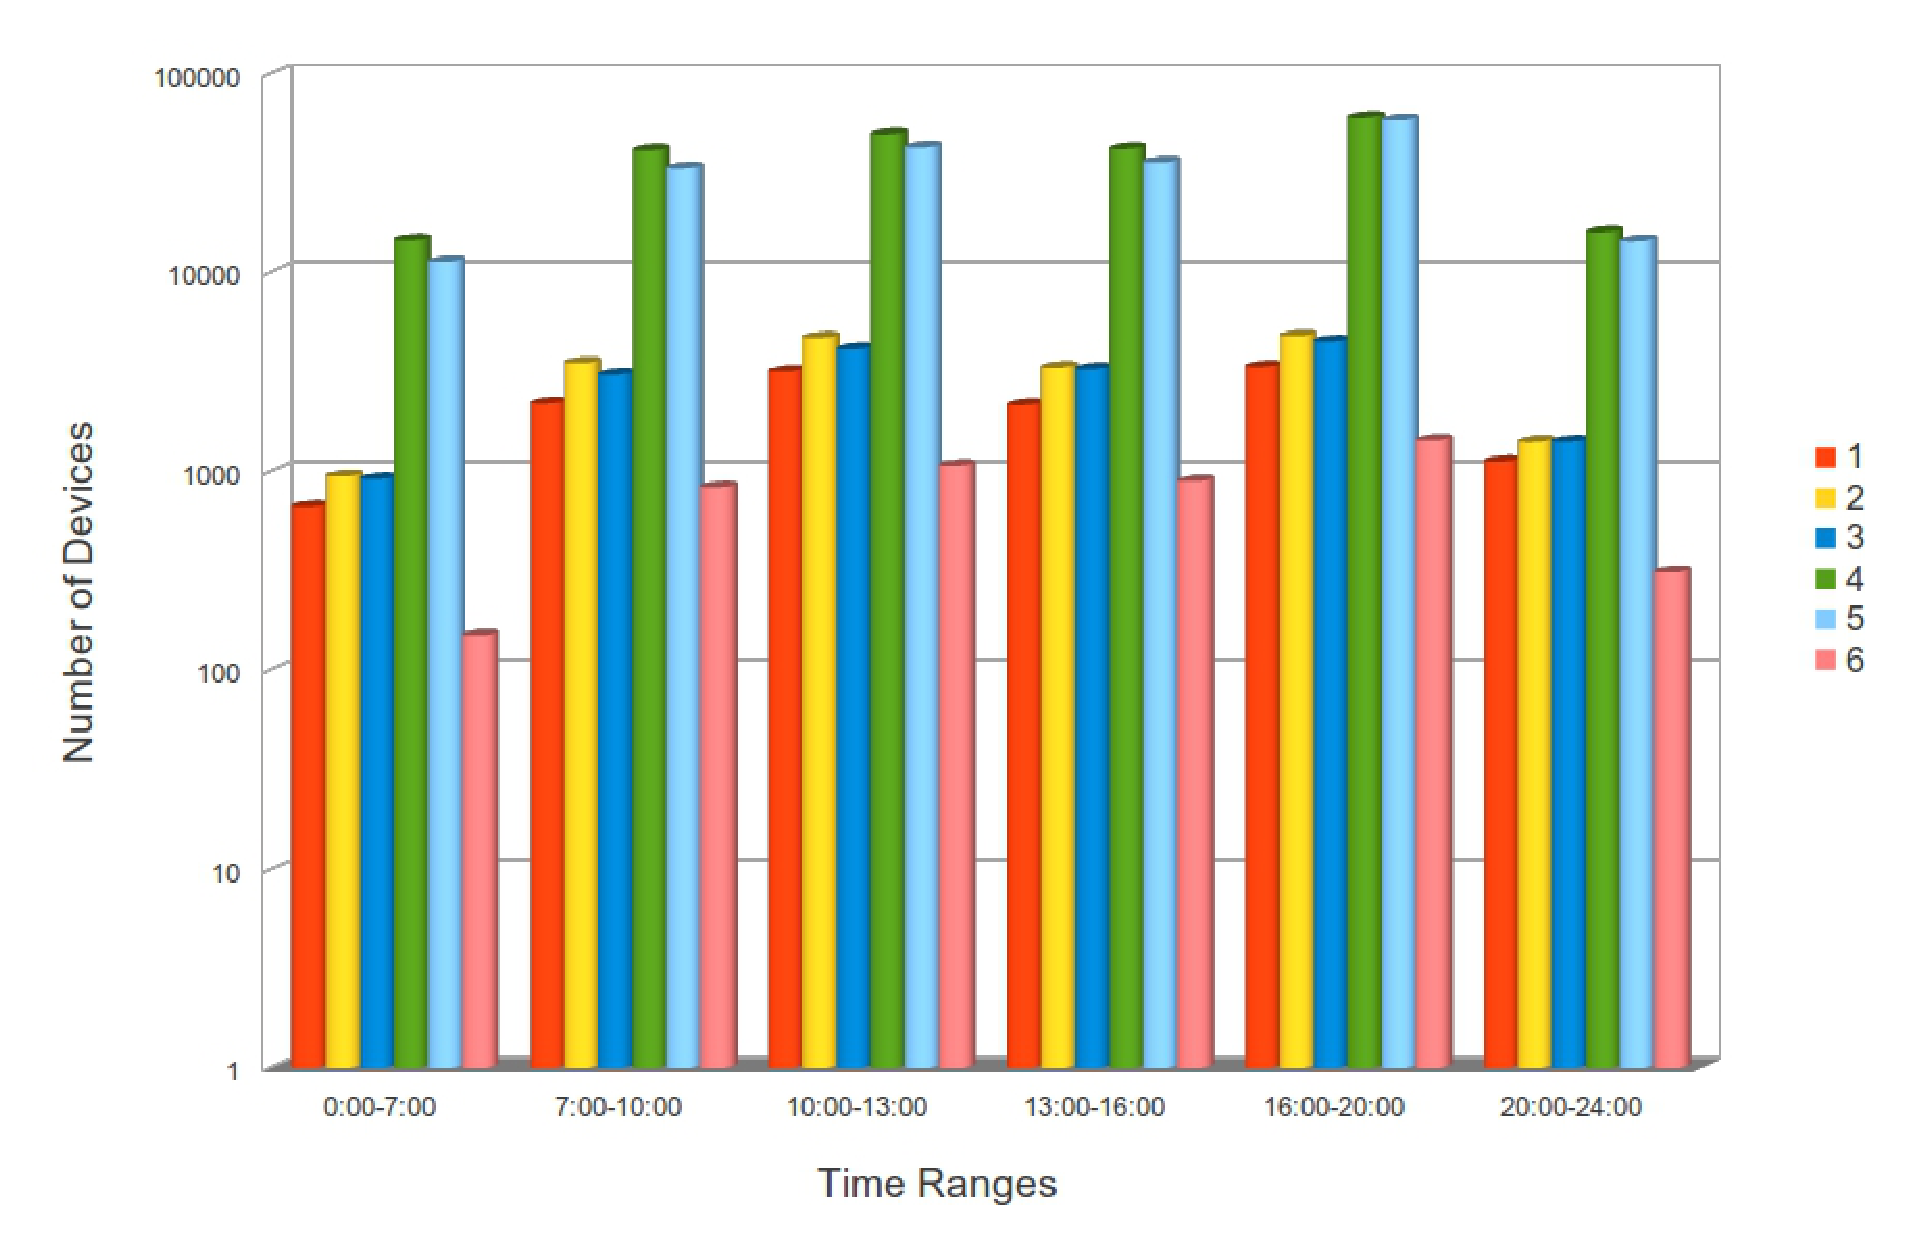
\includegraphics[scale=0.2]{images/Figure_5}
\end{center}
\end{figure}

Figure \ref{fig:f5} shows the number of individual detected devices in each node along the day and taking into account six time-ranges. 

As can be seen, a high density on all nodes is reached at peak times (7:00 to 10:00 and 16:00 to 20:00).
This might be due to the people going/returning to/from work and school, and those who are in leisure time.

This figure shows individual devices, eliminating repeated appearances of vehicles.

\subsection{Total detections by time range}
Additionally we can calculate for each node the number of detected devices by time range, without differentiating whether the device is the same or not (repeated passes). In this case, repeated appearances of vehicles have been taken into account (Figure \ref{fig:f6}).

\begin{figure}[ht]
\caption{For each of the six nodes, the total number of detected devices by time range is shown. Figure is shown in logarithmic scale.}
\label{fig:f6}
\begin{center}
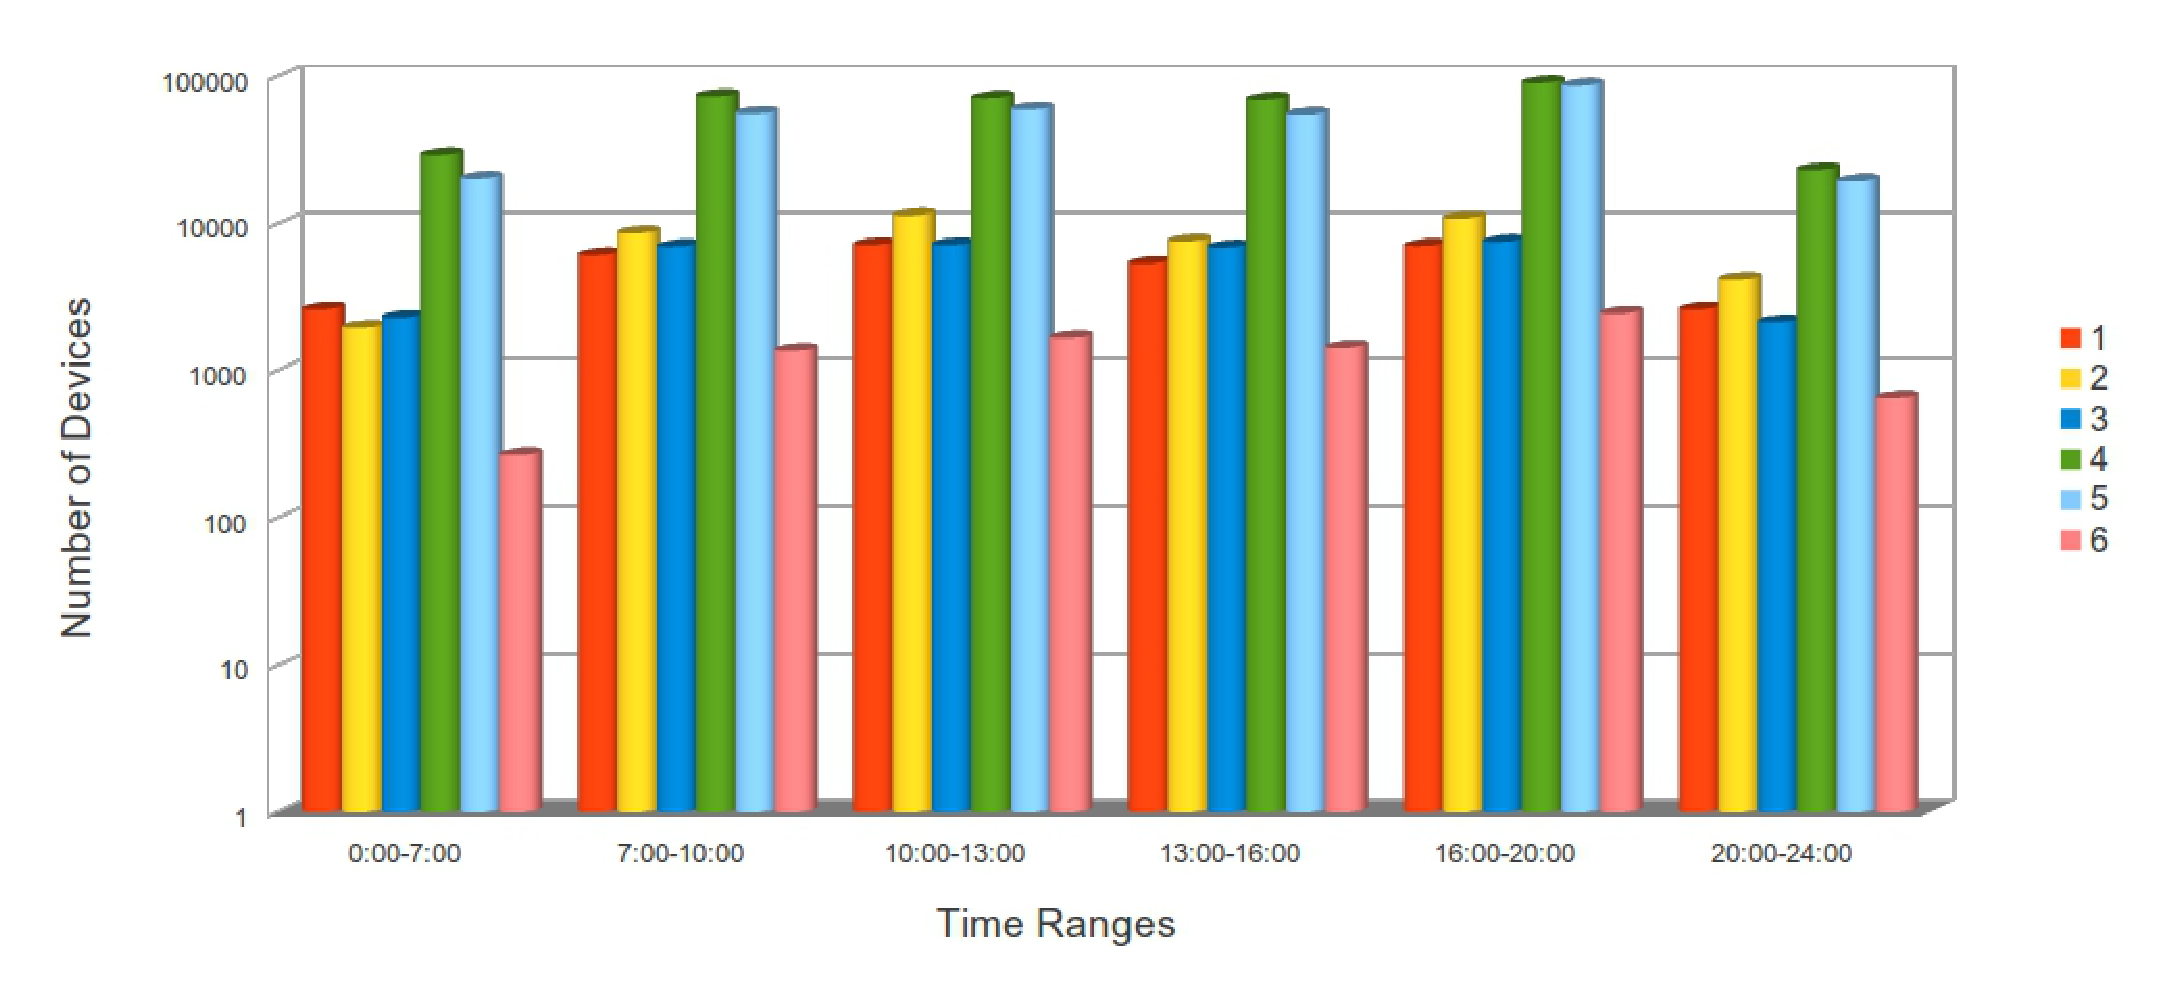
\includegraphics[scale=0.2]{images/Figure_6}
\end{center}
\end{figure}


Figure \ref{fig:f6} shows the total number of detected devices in each node along the day and taking into account six time-ranges. As in previous analysis (Figure 5), a high density on all nodes is reached at peak times (7:00 to 10:00 and 16:00 to 20:00).

\subsection{Number of individual vehicle detections}
We can take advantage of the proposed system's ability to identify BT devices. Thus, it can detect and report whether a vehicle pass by different nodes.

\begin{figure}[ht]
\caption{For each of the six nodes, the total number of detected devices N times (repeated occurrences of the same device) are shown. Figure is shown in logarithmic scale.}
\label{fig:f7}
\begin{center}
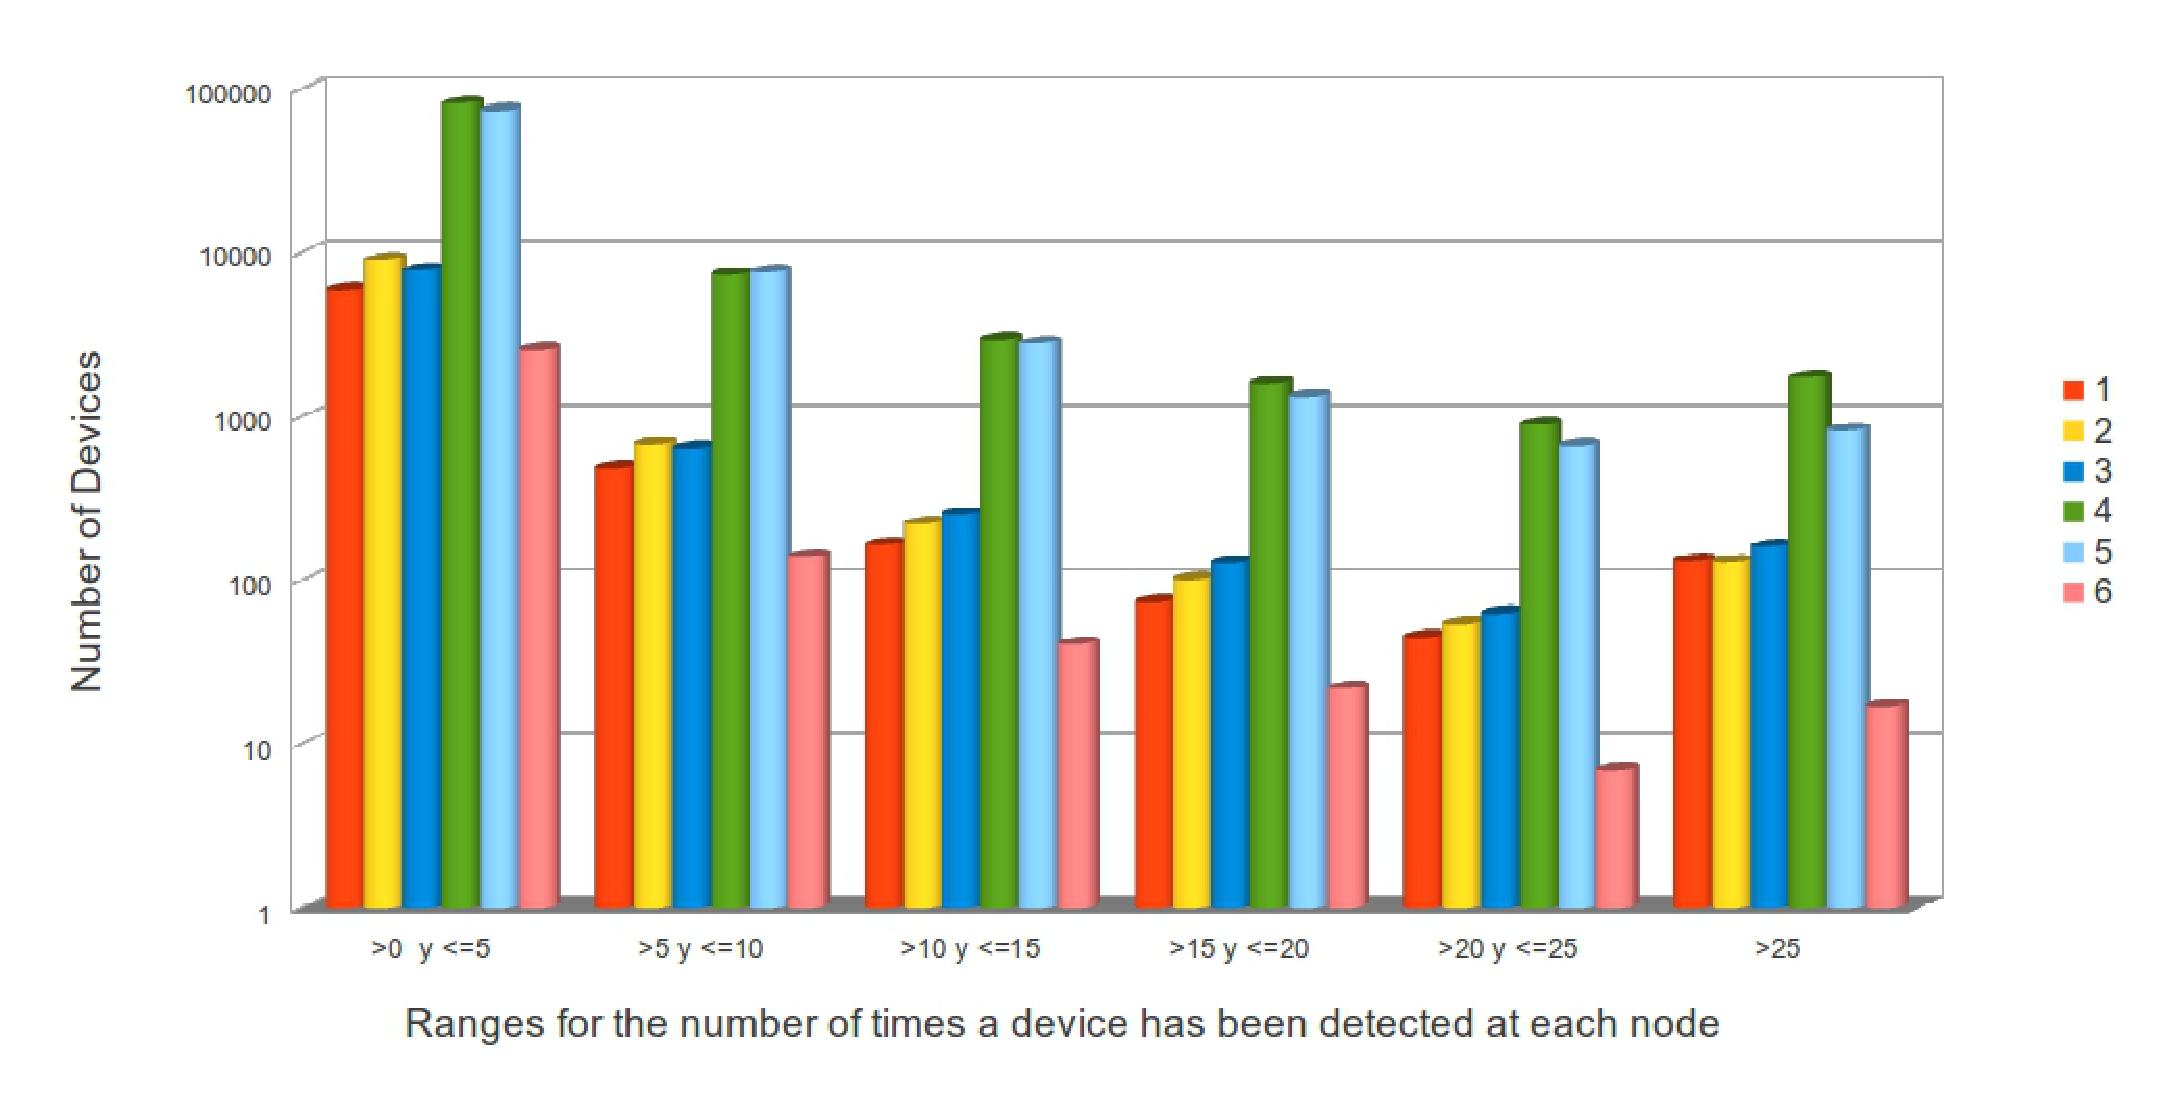
\includegraphics[scale=0.2]{images/Figure_7}
\end{center}
\end{figure}

This figure displays how many times an individual device has been detected in each node, i.e., if device A has been detected three times in node 4, then A is shown into the range ">0 \& <=5" for node 4.

Figure \ref{fig:f7} shows a large number of vehicles that pass repeated times (up to 10 times) by some of the nodes (mainly those located in the A44). Even, it can be seen that nodes 4 and 5 detect about 1,000 vehicles passing more than 25 times repeatedly, what means that many vehicles repeat their pass over and over again. Paying attention to the remainder nodes, over 25 repetitions of the same device have been detected only around 120 times.

Finally, as most of the devices have been detected only one time, then the first range >0 \& <=5 includes the largest number of detected devices.

\subsection{Complexity of displacements}

To study the complexity of displacements, the number of vehicles that have sequentially visited several nodes were calculated. Table \ref{table:complex} also shows the average number of times that vehicles have visited 2, 3, 4, 5 or 6 nodes.
\small {
\begin{table}

\caption{Total number of vehicles that have visited two nodes, 3 nodes and up to 6 nodes, and average number of times that vehicles have passed through 2, 3, 4, 5 or 6 nodes. In some cases the deviations are high due to the fact that some devices have a very high number of occurrences for some nodes.}
\label{table:complex}
\begin{center}
\begin{tabular}{|r|r|r|c|}\hline 
\bfseries Nodes & \bfseries  Devices & \bfseries Passes & \bfseries  Mean $ \pm $ std. dev.
\\\hline
\csvreader[head to column names, late after line=\\\hline]{Complexity.csv}{}
{ \nodes & \devices & \total & \mean }
\end{tabular}
\end{center}
\end{table}
}
Information in Table \ref{table:complex} is shown in Figure \ref{fig:f8}.

\begin{figure}[ht]
\caption{Complexity of displacements as the number of vehicles that have visited several nodes. Figure is shown in logarithmic scale.}
\label{fig:f8}
\begin{center}
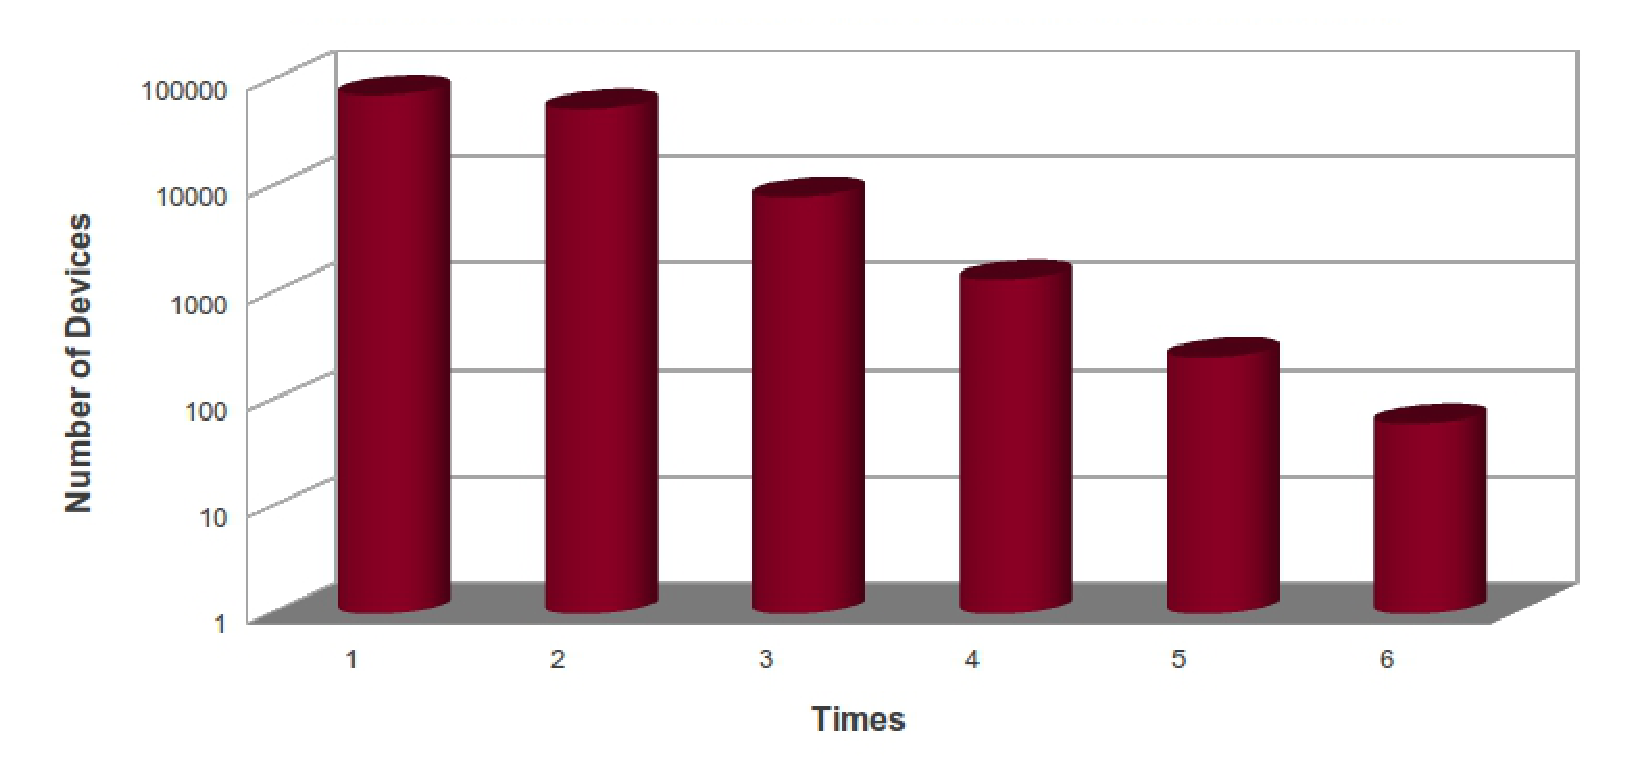
\includegraphics[scale=0.25]{images/Figure_8}
\end{center}
\end{figure}

As expected, most of the BT devices rarely visited all nodes sequentially, while most of devices pass only by one or two of nodes (their displacements are focused on a small part of the monitored area).

\subsection{Average speed on a section delimited by two consecutive nodes}
Finally, taking two consecutive nodes located on the A44 highway, average speeds in the section bounded by nodes 4 (located at km 119.550) and 5 (located at km 123.250) can be calculated. This highway section where the study takes place is 3700 meters long. Actually, we can calculate the average speed in the global section, but not the instant vehicle speed within that section (shown in Table \ref{table:speeds}).

\begin{table}
\caption{Average speeds (globally) in the section bounded by nodes 4 and 5.}
\label{table:speeds}
\begin{center}
\begin{tabular}{|C{3cm}|R{3cm}|}\hline 
\bfseries  Speed range (km/h) & \bfseries  \makebox[3cm][c]{N. of passes}
\\\hline
\csvreader[head to column names, late after line=\\\hline]{Speed.csv}{}
{ \speed & \passes }
\end{tabular}
\end{center}
\end{table}

In that section, the speed is limited to 100 km/h. As can be seen, although most of the vehicles respect this limit, a lot of them exceed this limitation.

In the other hand, this analysis has allowed us to detect slow traffic and even jams. In a near future, mobile application users could receive alerts in case of traffic events. Additionally, the information system is configured to store the exact time when a device is first detected and the exact time when it is no longer detectable. Thus, if a device is detected for a time longer than a specified number of seconds, that means slow traffic.

\section{Future research directions}

Among future improvements to the system, as hardware device, one based on the architecture of Raspberry-Pi will be used, as it is more energy efficient and cheaper. Thus, reducing costs installing new nodes is expected. The hardware team may perform this hardware device evolution and migration to the new model with minimal effort and independently of the software development team.

Additionally, the mobile application to serve information will be improved, allowing users to receive, not only numeric and graphic data, but also alerts on traffic events, such as slow traffic.

Several future research lines have been opened. They are mainly focused on processing the collected data using data mining algorithms \cite{hastie2005elements}, evolutionary computation methods \cite{eiben2003introduction}\cite{michalewicz2004solve}\cite{yang2010nature}, artificial neural networks \cite{castillo2001function}\cite{rivas2003evolving}\cite{castillo2007comparing}, machine learning models \cite{arenas2005co} and statistical methods \cite{han2006data}\cite{lewicki2006statistics}\cite{nisbet2009handbook}, which will be included and integrated as web services \cite{papazoglou2007service}\cite{} in the system.

A critical task that any new intelligent transportation system should face is short-term traffic flow prediction. Thus, our purpose is to develop in the future a prediction system that helps to make decisions, and able to apply knowledge in applications related to mobility. In this sense, different time series prediction methods will be used in order to estimate the vehicle passing. Time series forecasting is usually tackled trying to find out an underlying model that describes the series behaviour. Our system will test a variety of methods and include some of them to perform forecast, using both linear and nonlinear models \cite{brown1959statistical}\cite{winters1960forecasting}\cite{box2013time}\cite{Tong1978575}\cite{qiu2011generalized}\cite{wang2011comparison}\cite{rivas2004evolving}. 

It is expected that the development and deployment of these systems will offer a set of information services with added value that can not be achieved with current technologies. 

\section{Conclusion}

The information systems currently used for collecting data about the road conditions are not able to identify detected vehicles, and if they do, these information systems have a high cost.

In this chapter a new low-cost information system to monitor traffic on different road types and in real time has been presented.

The main goal was getting exposure indicators using a new system based on the BT devices detection using several collecting nodes. This way, both the traffic density and car journeys have been monitored, identifying the vehicles when they move from one node to another inside the monitored zone.

Moreover, different hardware solutions have been studied to carry out device detection; some of them have been rejected due to their high prices, due to their energy inefficiency or due to their short-range for detection.

In this study, different road types, with different traffic type have been taken into account. Statistical data have also been obtained grouped by days of the week and hours of day.

Several statistics of the collected data have been calculated during the monitoring period (November 8th to December 9th, 2012). Specifically, the total number of BT detected devices by each node has been analyzed, on holidays or working days. We also have analyzed the traffic density by time range, and the journeys in the monitored zone. As a final analysis, the average speed on a highway section delimited by two consecutive nodes has been obtained, allowing us to detect slow traffic.

Finally, the power and features of the system have been demonstrated. This has been complemented by developing a set of web services based on Google Fusion Tables for easy access to the data in real time, including different statistics.



\section*{Agradecimientos}

This work is supported in part by the 0100DGT21285 project of the Spanish Direccio?n General de Tra?fico, and the FEDER of European Union project "Sistema de Informaci�n y Predicci�n de bajo coste y aut�nomo para conocer el Estado de las Carreteras en tiempo real mediante dispositivos distribuidos SIPEsCa  ? G-GI3000/IDIF? (Programa Operativo FEDER de Andaluc�a 2007-2013). We also thank all Agency of Public Works of Andalusia Regional Government staff and researchers for their dedication and professionalism. The authors are very grateful to the anonymous referees whose comments and suggestions have contributed to improve this paper.

\begin{figure}[ht]
\label{fig:f9}
\begin{center}

\includegraphics[scale=0.85]{images/Figure_9}
\end{center}
\end{figure}

\nocite{*}
\bibliographystyle{Jornadas}
\bibliography{bibliografia}

\end{document}

